\chapterimage{banalisis.jpg}
\chapter{Análisis}
\begin{figure}[th!]
	\centering
	\includegraphics[width=0.4\linewidth]{analisis}
\end{figure}
\section{Introducción}
El análisis de los requerimientos puede ser uno de los procesos más complejos que se presentan a la hora de desarrollar un programa de software, esto se debe a que muchas veces no basta con entender el problema y la posible solución para este, sino que igualmente es necesario comprender las necesidades del cliente, saber qué es lo que quiere, pero muchas veces es el mismo cliente el que no sabe esto último, lo cual complica bastante el proceso.
\newline
\newline
Realizar un buen análisis del proyecto nos garantiza una base solida para la elaboración de nuestro producto, de ahí que sea una de las partes más importante, quizá la más importante, a la hora de realizar un proyecto, ya que es nuestro punto de partida, la forma que tenemos para guiarnos durante el proceso de desarrollo, los planos de nuestro proyecto, por lo que sin el análisis inicial lo más probable es que se este destinado al fracaso.
\newpage

\section{Diagrama de Casos de Uso}

\begin{figure}[th!]
	\centering
	\includegraphics[width=1\linewidth]{Casodeuso}
    \caption{Caso de uso del sistema de gestión de monitorias}
	\label{fig:Casodeuso}
\end{figure}

\begin{table}[H]
\centering
\begin{tabular}{|l|l|l|l|}
\hline
\textbf{Nombre:}        & Sustituir papeleo físico                                                      & \textbf{Id:}                                                    & CU01                                                   \\ \hline
\textbf{Actores:}       & \multicolumn{3}{l|}{Monitor, Profesor}                                                                                                                                                                   \\ \hline
\textbf{Objetivo:}      & \multicolumn{3}{l|}{Agilizar la certificación de la monitoria}                                                                                                                                           \\ \hline
\multicolumn{4}{|c|}{\textbf{Escenarios}}                                                                                                                                                                                          \\ \hline
\textbf{Primario:}      & \multicolumn{3}{l|}{Digitalizar toda la documentación requerida en el proceso}                                                                                                                                 \\ \hline
\textbf{Secundario:}    & \multicolumn{3}{l|}{\begin{tabular}[c]{@{}l@{}}-Documentación incompleta\\ -Horas incompletas\\ -Objetivos incompletos\end{tabular}}                                                                     \\ \hline
\textbf{Excepcionales:} & \multicolumn{3}{l|}{\begin{tabular}[c]{@{}l@{}}-Tamaño virtual de los soportes muy grande \\ -Formato de los soportes incompatible\\ -Falta de comunicación\\ -Inconsistencia en los datos

\end{tabular}} \\ \hline
\end{tabular}
\caption{Especificaciones de caso de uso 01}
\label{tab:EspecificacionCu01}
\end{table}

\begin{table}[H]
\centering
\begin{tabular}{|l|l|l|l|}
\hline
\textbf{Nombre:}        & \begin{tabular}[c]{@{}l@{}}Establecer una comunicación oportuna\\ en el proceso.\end{tabular}                      & \textbf{Id:}                     & CU02                    \\ \hline
\textbf{Actores:}       & \multicolumn{3}{l|}{Monitor, Profesor, Coordinador}                                                                                                                              \\ \hline
\textbf{Objetivo:}      & \multicolumn{3}{l|}{\begin{tabular}[c]{@{}l@{}}Contribuir a la interacción entre los actores del \\ sistema\end{tabular}}                                                        \\ \hline
\multicolumn{4}{|c|}{\textbf{Escenarios}}                                                                                                                                                                  \\ \hline
\textbf{Primario:}      & \multicolumn{3}{l|}{Visualizar la información de contacto de los actores}                                                                                                        \\ \hline
\textbf{Secundario:}    & \multicolumn{3}{l|}{\begin{tabular}[c]{@{}l@{}}-Inexistencia de datos registrados\\ -Información de contacto incompleta\\ -Inconsistencia de los datos de contacto\end{tabular}} \\ \hline
\textbf{Excepcionales:} & \multicolumn{3}{l|}{\begin{tabular}[c]{@{}l@{}}-Fallo en la persistencia de los datos\\ -Falla de comunicación\end{tabular}}                                                     \\ \hline
\end{tabular}
\caption{Especificaciones de caso de uso 02}
\label{tab:EspecificacionCu02}
\end{table}

\begin{table}[H]
\centering
\begin{tabular}{|l|l|l|l|}
\hline
\textbf{Nombre:}        & Reducir tiempo de tramite                                                             & \textbf{Id:}                                                         & CU03                                                         \\ \hline
\textbf{Actores:}       & \multicolumn{3}{l|}{Monitor, Profesor, Coordinador}                                                                                                                                                                         \\ \hline
\textbf{Objetivo:}      & \multicolumn{3}{l|}{Contribuir a la rápida certificación de monitores}                                                                                                                                                      \\ \hline
\multicolumn{4}{|c|}{\textbf{Escenarios}}                                                                                                                                                                                                             \\ \hline
\textbf{Primario:}      & \multicolumn{3}{l|}{\begin{tabular}[c]{@{}l@{}}Generar informe de certificación dentro de fechas\\ preestablecidas\end{tabular}}                                                                                            \\ \hline
\textbf{Secundario:}    & \multicolumn{3}{l|}{-Vencimiento de plazo para la certificación}                                                                                                                                                            \\ \hline
\textbf{Excepcionales:} & \multicolumn{3}{l|}{\begin{tabular}[c]{@{}l@{}}-Falta de oportunidades para completar las horas/\\ objetivos\\ -Retraso en el cumplimiento de las tareas.\\ -Fallas en el calendario del servidor del sistema\end{tabular}} \\ \hline
\end{tabular}
\caption{Especificaciones de caso de uso 03}
\label{tab:EspecificacionCu03}
\end{table}

\newpage

\section{Interacciones}
Todos los sistemas incluyen interacciones de algún tipo. Éstas son interacciones del usuario, que implican entradas y salidas del usuario; interacciones entre el sistema a desarrollar y otros sistemas; o interacciones entre los componentes del sistema. El modelado de interacción del usuario es importante, pues ayuda a identificar los requerimientos del usuario. El modelado de la interacción sistema a sistema destaca los problemas de comunicación que se lleguen a presentar. El modelado de interacción de componentes ayuda a entender si es probable que una estructura de un sistema propuesto obtenga el rendimiento y la confiabilidad requeridos por el sistema.\cite{modeladosistema}

Los diagramas de interacción de más frecuente uso son los siguientes:
\begin{itemize}
\item Diagrama de Secuencia
\begin{figure}[H]
	\centering
	\includegraphics[width=0.7\linewidth]{diagsec}
    \caption{Ejemplo de diagrama de secuencia}
	\label{fig:dseEjemplo}
\end{figure}
\item Diagrama de Comunicación
\begin{figure}[H]
	\centering
	\includegraphics[width=0.7\linewidth]{diagcom}
    \caption{Ejemplo de diagrama de comunicaciones}
	\label{fig:dcomEjemplo}
\end{figure}
\end{itemize}
\newpage
\subsection{Diagrama de Secuencia}
El diagrama de secuencia es un tipo de diagrama usado para modelar interacción entre objetos
en un sistema. Este tipo de diagrama muestra la interacción de un conjunto de objetos en una aplicación
a través del tiempo y se modela para cada caso de uso. Mientras que el diagrama de casos de uso
permite el modelado de una vista del negocio para el escenario, el diagrama de secuencia contiene detalles
de implementación del escenario, incluyendo los objetos y clases que se usan para implementar el
escenario y mensajes intercambiados entre los objetos.

A continuación se muestran algunos de los escenarios más importantes de las interacciones del sistema:
\begin{figure}[th!]
	\centering
	\includegraphics[width=1\linewidth]{patronlogueo}
    \centering
    \caption{Diagrama de secuencia para la autenticación de un usuario en el sistema}
	\label{fig:patronlogueo}
\end{figure}

En el anterior diagrama de secuencia sucede lo primero que debe hacer un usuario antes de hacer uso de las funcionalidades del sistema: autenticarse como un usuario, este usuario es único y tiene distintas funcionalidades dependiendo de su rol. 
\clearpage
Por ejemplo en el siguiente diagrama de secuencia se muestra la funcionalidad del escenario primario del caso de uso 03 apreciado en el cuatro 3.3, donde el coordinador se encarga de generar los certificados de cada monitor.

\begin{figure}[H]
	\centering
	\includegraphics[width=1\linewidth]{diagseqcertificado}
    \caption{Diagrama de secuencia para la certificación de las monitorías}
	\label{fig:dsecertificacion}
\end{figure}

Por otro lado una funcionalidad clave del sistema es permitir el contacto oportuno entre los usuarios del sistema, observado en el caso de uso 02 del cuadro 3.2. En este diagrama de secuencia se generaliza primordialmente para todos los usuarios, pues todos tienen la posibilidad de visualizar bien sea el correo o el teléfono de los involucrados en el proceso.
\begin{figure}[H]
	\centering
	\includegraphics[width=1\linewidth]{dsecontacto}
    \caption{Diagrama de secuencia para el contacto entre usuarios del sistema}
	\label{fig:dsecontacto}
\end{figure}

Ahora, existirán situaciones en las que un docente necesita de ayuda extra dentro de la academia, y un estudiante necesita horas para poder certificarse, es en este escenario donde el docente puede publicar un clasificado en el sistema a la espera de que algún estudiante lo contacte, a continuación se visualiza esta situación en un diagrama de secuencia: 
\begin{figure}[H]
	\centering
	\includegraphics[width=1\linewidth]{dseclasificados}
    \centering
    \caption{Diagrama de secuencia para la publicación de clasificados por parte del profesor}
	\label{fig:dseclasificados}
\end{figure}

En el siguiente diagrama de secuencia puede que describamos uno de los procesos más fundamentales de nuestro aplicativo, el hecho de permitirle a el docente poder llevar un registro de las horas de los monitores a su cargo es algo esencial, por ello nuestro actor principal en esta abstracción sera el docente, aquel que tiene acceso a una interfaz gráfica que le luego le permitirá seleccionar a un estudiante, por medio de una petición la interfaz accede  al control para que este posteriormente, pueda acceder a la base de datos de los estudiantes y pueda regresar información sobre las horas de monitoria de un estudiante, al obtener esta información en un proceso inmediatamente continuo, se desplegara en la interfaz esta información, para que el docente pueda modificarla, es decir para que el docente tenga la capacidad de llenar las horas que le hacen falta al estudiante. De este modo nos aseguramos de una total transparencia en el proceso, ademas de el hecho de ahorrarnos un montón de papeleo y firmas innecesarias:
\begin{figure}[H]
	\centering
	\includegraphics[width=1\linewidth]{horas}
    \centering
    \caption{Diagrama de secuencia para la certificación de horas de monitoría}
	\label{fig:dsehoras}
\end{figure}

El diagrama de digitalización de los documentos nos describe una automatización y visualización virtual, completa de los documentos que se tienen que presentar en los procesos de monitorias, para ello haremos uso de una base de datos que lleve registro de cada uno de los estudiantes implicados en las monitorias, como es obvio nuestro actor principal sera el estudiante, para ser exactos los monitores, ellos podrán acceder a la plataforma mediante sus cuentas, en donde encontraran una interfaz que les permitirá llenar su información principal y donde podrán subir todo documento requerido, para ello deberán subir una imagen de dichos requisitos, la cual sera llevada a un control que procederá a guardar la en la base de datos, si no hay errores externos, la plataforma le verificara al estudiante el estado de su  información:
\begin{figure}[H]
	\centering
	\includegraphics[width=1\linewidth]{digidoc}
    \centering
    \caption{Diagrama de secuencia para la digitalización de documentos}
	\label{fig:dsedigidoc}
\end{figure}


\newpage

\subsection{Diagrama de Comunicación}
Un diagrama de comunicación nos permite modelar las distintas interacciones y acciones entre objetos de nuestro proyecto, normalmente son combinaciones de información de otro tipo de diagramas tales como el de clases o el de secuencia que previamente hemos realizado, este nos ayuda a describir el comportamiento de nuestro sistema por medio de mensajes, por ello es normal que el nombre de los objetos del diagrama de comunicación sean los mismo que los del diagrama de secuencia, estos mensajes al igual que en el anterior diagrama están organizados por importancia a la hora de ser realizados, no podemos acceder a una base de datos si previamente no nos identificamos con el sistema.

En el siguiente diagrama de comunicación podemos ver el proceso del sistema a la hora de ingresar al sistema, pero podemos observar un cambio en el control  al acceso de la base de datos, como podemos ver en este objeto tenemos un mensaje que esta redireccionando a si mismo, es decir que este tiene la capacidad de validar antes de devolver la información a la interfaz, esto es esencial en aplicativo debido a que si no pensáramos en este tipo de control, en un nivel alto de nuestra aplicación cualquiera podría acceder a los datos y dañar nuestra información. 

\begin{figure}[H]
	\centering
	\includegraphics[width=0.8\linewidth]{dcomLogin}
    \centering
    \caption{Diagrama de comunicación para el diagrama de secuencia de la figura 3.2}
	\label{fig:dcomLogin}
\end{figure}
\clearpage
Cada doble mensaje que observamos nos permite visualizar una acción que toma nuestro sistema, aun y sin embargo este diagrama no nos permite visualizar los mensajes de retorno, esto se debe a que estos diagramas de comunicación son un complemento de nuestro proceso de abstracción, en este caso nos retornaría la información del estudiante. 
\begin{figure}[H]
	\centering
	\includegraphics[width=0.8\linewidth]{dcomCertifi}
    \centering
    \caption{Diagrama de comunicación para el diagrama de secuencia de la figura 3.3}
	\label{fig:dcomCertifi}
\end{figure}
\clearpage
El siguiente diagrama de comunicación refleja la secuencia de mensajes realizada por el programa para permitir al usuario obtener la información necesaria, en este caso la información de contacto de otro usuario, que puede ser profesor o monitor y con lo que se garantizaría la oportuna comunicación entre los diferentes usuarios de la aplicación. 
\begin{figure}[H]
	\centering
	\includegraphics[width=0.8\linewidth]{dcomContacto}
    \centering
    \caption{Diagrama de comunicación para el diagrama de secuencia de la figura 3.6}
	\label{fig:dcomContacto}
\end{figure}
\clearpage
Del mismo modo la siguiente figura ilustrar la forma en la que el programa permite a un docente buscar un monitor disponible, por medio de un clasificado que será guardado y posteriormente mostrado a los demás usuarios, específicamente a los monitores que estén disponibles para completar sus horas de monitoria.
\begin{figure}[H]
	\centering
	\includegraphics[width=0.8\linewidth]{dcomClasifi}
    \centering
    \caption{Diagrama de comunicación para el diagrama de secuencia de la figura 3.7}
	\label{fig:dcomClasifi}
\end{figure}
\clearpage
El siguiente diagrama de comunicación nos da a conocer las direcciones de los mensajes entre los distintos objetos, desde el profesor y seleccionar a un estudiante y agregarle las horas correspondientes por su labor de monitorias, lo cual lo realiza mediante un objeto interface, este nos permite representar la parte grafica de nuestra app, a su vez conectado por un objeto control, este se encarga de transmitir la información capturada en el objeto que interactúa con el actor principal, haciendo las veces de puente entre una interface y una persistencia, este referencia la información a nuestro objeto base de datos (BD) este realiza la función de consulta y modificación de la base, mediante los mensajes de consultar datos del estudiante y guardar las horas.
\begin{figure}[H]
	\centering
	\includegraphics[width=0.7\linewidth]{dcomHoras}
    \centering
    \caption{Diagrama de comunicación para el diagrama de secuencia de la figura 3.6}
	\label{fig:dcomHoras}
\end{figure}
\clearpage
Este diagrama de comunicación es el que nos permite la virtualización en gran parte del papeleo, para ello el actor principal en este caso un estudiante, al llenar su información personal, junto con algunos archivos específicos e imágenes, interactúa con un objeto Interface, aquel le permite al usuario digitar y capturar sus datos para evitar todo tramite presencial y molesto, mediante el mensaje subir documento, se planea capturar toda información de un estudiante para luego ser llevada a un control que se encargue mediante otro enlace de comunicación de decirle al objeto BD, que es el que interactúa directamente con nuestra base de datos, que actualice cierta información, dado cierto punto del proceso, el actor solo podrá actualizar su información, ya que la modificación de sus datos personales solo será supervisada por un actor externo de mayor jerarquía, esto con el fin de evitar información corrupta
\begin{figure}[H]
	\centering
	\includegraphics[width=0.7\linewidth]{dcomDigi}
    \centering
    \caption{Diagrama de comunicación para el diagrama de secuencia de la figura 3.7}
	\label{fig:dcomDigi}
\end{figure}
\clearpage

\newpage

\subsection{Diagrama de Temporización}

\newpage

\section{Diagramas de Actividades}

\newpage

\section{Diagramas de Workflow}

Workflow es la automatización de un proceso de negocio, sea parcial o totalmente, durante el cual documentos, información o tareas son pasados desde un participante a otro para la ejecución de otra acción, de acuerdo a un conjunto de reglas procedurales. \cite{workflow} Para el caso del Sistema de Gestión de Monitorías se pueden destacar los siguientes procesos:

\begin{figure}[H]
	\centering
	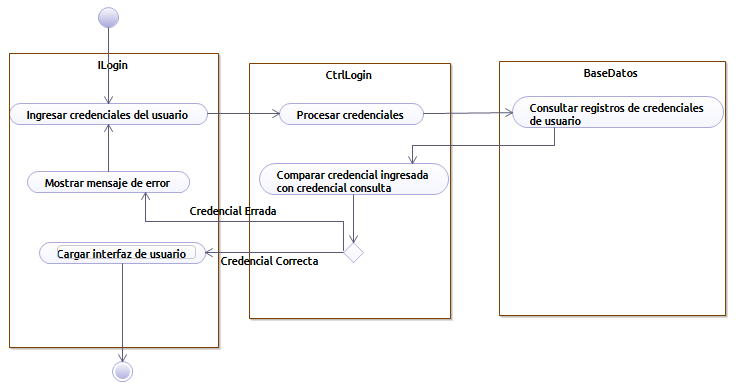
\includegraphics[width=0.9\linewidth]{wfLogin}
	\centering
	\caption{Diagrama de workflow para la autenticación de usuarios.}
	\label{fig:wfLogin}
\end{figure}
\begin{figure}[H]
	\centering
	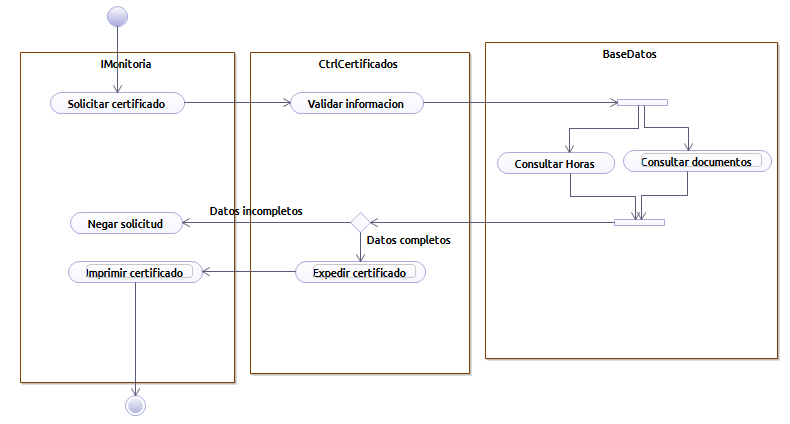
\includegraphics[width=0.9\linewidth]{wfCertificado}
	\centering
	\caption{Diagrama de workflow para la certificación de monitorias.}
	\label{fig:wfCertificado}
\end{figure}
\clearpage
\begin{figure}[H]
	\centering
	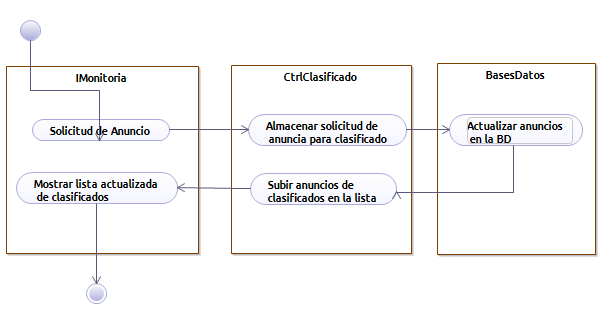
\includegraphics[width=0.9\linewidth]{wfClasificado}
	\centering
	\caption{Diagrama de workflow para los clasificados y anuncios.}
	\label{fig:wfClasificado}
\end{figure}
\begin{figure}[H]
	\centering
	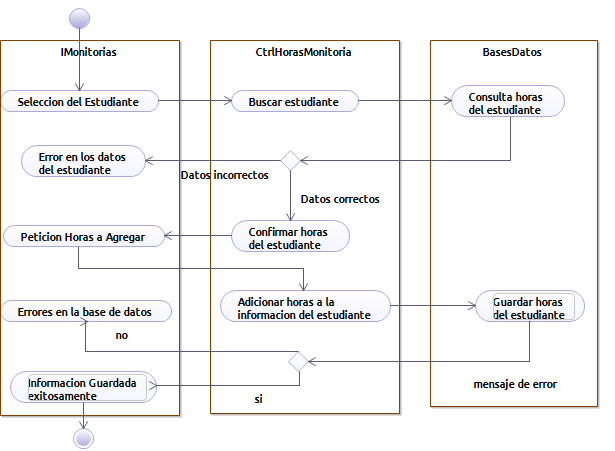
\includegraphics[width=0.9\linewidth]{wfHorasMonitoria}
	\centering
	\caption{Diagrama de workflow para la certificación de Horas.}
	\label{fig:wfHorasMonitoria}
\end{figure}
\clearpage
\begin{figure}[H]
	\centering
	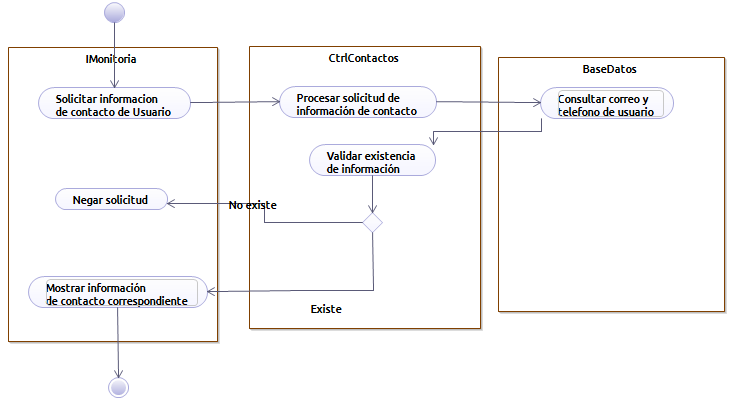
\includegraphics[width=0.9\linewidth]{wfContacto}
	\centering
	\caption{Diagrama de workflow para el contacto de usuarios.}
	\label{fig:wfContacto}
\end{figure}

\newpage

\section{Diagramas de Descripción de la Interacción}

\newpage

\section{Diagramas de Estado}
El diagrama de estado es una representación particular de las fases que se pueden presentar un proyecto, encaminado a la abstracción que posee el mismo dado que estas faces resumen ampliamente el comportamiento de nuestras aplicaciones, en verdad son las condiciones y ciclo de vida en general de un objeto. 
Dado que nos podría dar información explicita del ciclo de vida de nuestro objeto, también nos permite conocer su naturaleza, la relación y transición entre las fuentes y objetivos se hacen más fáciles de interpretar.
Normalmente este tipo de transiciones se componen de la fuente, un disparo, una condición, una acción y por ultimo una fuente, a través de comparaciones es que se logra la representación de algoritmos y por ende de cambios de estado.  
Los estados se representan por medio de rectángulos redondeados que se etiquetan con el nombre del estado, mientras que las transiciones se marcan con flechas que fluyen de un estado a otro representando el cambio de uno a otro.
\begin{figure}[H]
	\centering
	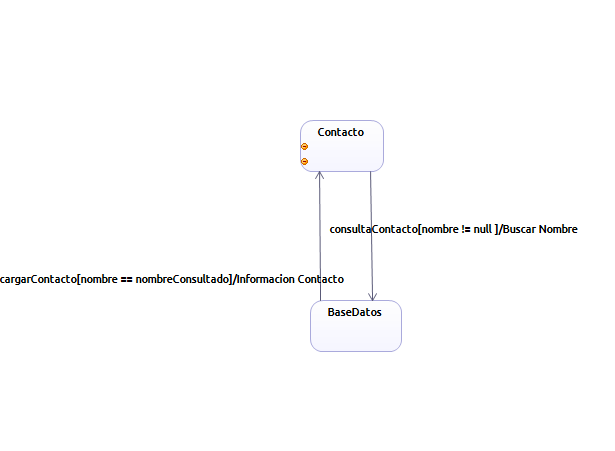
\includegraphics[width=0.9\linewidth]{desContacto}
	\centering
	\caption{Diagrama de Estado para el contacto entre Docente/Monitor).}
	\label{fig:desContacto}
\end{figure}

\begin{figure}[H]
	\centering
	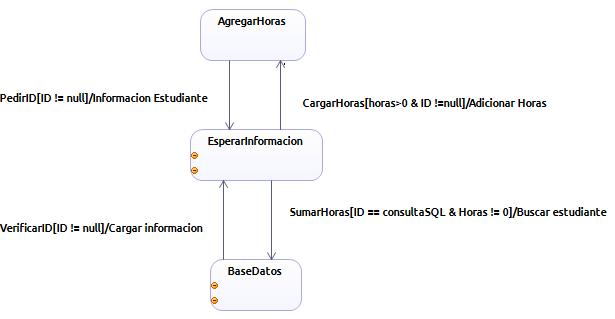
\includegraphics[width=0.9\linewidth]{desCertificarHoras}
	\centering
	\caption{Diagrama de Estado para la certificación de Horas.}
	\label{fig:desCertificarHoras}
\end{figure}
\newpage